\documentclass[11pt,twoside]{article}
\usepackage{geometry}
\usepackage{enumerate}
\usepackage{latexsym,booktabs}
\usepackage{amsmath,amsthm,amssymb}
\usepackage{graphicx}
\usepackage{natbib}
\usepackage[singlespacing]{setspace}
\usepackage{subcaption}
\usepackage{listings}
\usepackage{xcolor}
%
\lstset{
language=R,
basicstyle=\scriptsize\ttfamily,
commentstyle=\ttfamily\color{gray},
numbers=left,
numberstyle=\ttfamily\color{gray}\footnotesize,
stepnumber=1,
numbersep=5pt,
backgroundcolor=\color{white},
showspaces=false,
showstringspaces=false,
showtabs=false,
frame=single,
tabsize=2,
captionpos=b,
breaklines=true,
breakatwhitespace=false,
title=\lstname,
escapeinside={},
keywordstyle={},
morekeywords={}
}
%
%
%
%
%
%
%
\geometry{a4paper,left=3cm,right=2.0cm, top=2cm, bottom=2.0cm}
%
\newtheorem{Definition}{Definition}
\newtheorem{Theorem}{Theorem}
\newtheorem{Lemma}{Lemma}
\newtheorem{Corollary}{Corollary}
\newtheorem{Proposition}{Proposition}
\newtheorem{Algorithm}{Algorithm}
\numberwithin{Theorem}{section}
\numberwithin{Definition}{section}
\numberwithin{Lemma}{section}
\numberwithin{Algorithm}{section}
\numberwithin{equation}{section}
%
%
\begin{document}
%
\pagestyle{empty}
%
% =============================================================================
% Title page
% =============================================================================
\begin{titlepage}
\vspace*{.5em}
\center
\textbf{\large{The School of Mathematics}} \\
\vspace*{1em}
\begin{figure}[!h]
\centering
\includegraphics[width=180pt]{CentredLogoCMYK.jpg}
\end{figure}
\vspace{2em}
\textbf{\Huge{Liver Cancer: Investigating the Risk Factors}}\\[2em]
\textbf{\LARGE{by}}\\
\vspace{2em}
\textbf{\LARGE{Eric Roseren, s1786435}}\\
\vspace{6.5em}
\vspace{6.5em}
\Large{July 2018}\\
\vspace{3em}
\normalsize{Supervised by\\Dr Vanda Inacio de Carvalho, Prof Ruth King and Dr Ruben Amoros Salvador}
\vfill
\end{titlepage}
%
\clearpage
%
% =============================================================================
% Acknowledgments, and own work declaration
% =============================================================================
%
% \begin{center}
% \Large{Acknowledgments}
% \end{center}
%
% Here come your acknowledgments ...
%
% \clearpage
%
\begin{center}
\Large{Own Work Declaration}
\end{center}
I confirm that the work contained in this report was solely undertaken by myself and that no help was provided from other sources as those allowed. All sections of the report that use quotes or describe an argument or concept developed by another author have been referenced, including all
secondary literature.%
\cleardoublepage
%
%
%
% =============================================================================
% Table of contents, tables, and pictures (if applicable)
% =============================================================================
\pagestyle{plain}
\setcounter{page}{1}
\pagenumbering{Roman}
%
\cleardoublepage
%
\pagenumbering{arabic}
\setcounter{page}{1}
%
%
\clearpage
\section*{Executive summary}
\addcontentsline{toc}{section}{Executive summary}

Hepatocellular Carcinoma (HCC) is currently the second leading cause of cancer-related death in the world. It is recognised that over $90\%$ of diagnosed HCC are linked to cirrhosis. Several factors has been identified as damaging the liver and causing cirrhosis. This report will aim to explain the different risk factors associated with five different pre-conditional diseases.\\ \\
%
%
In the first part of the report, we started by assessing the impact of gender and the different aetiologies on the incidence of HCC using a multivariate Cox regression model. We found that female patients had better survival outcome than males and that for both male and female, poorer survival outcome arises in patients with Hepatitis C and NAFLD followed by ALD.
%
%
Additionally, this project proposes a model to estimate the survival probabilities of a patient after each new measurement taken. The model uses a joint modelling approach which combines two sub-models a longitudinal model and a survival model. The longitudinal model constructs a longitudinal profile for each patient whereas the survival model evaluates hazard ratio for a set of predictors. The goal is then to assess the degree of association between the biomarker's trend and event time.
Our results indicated a strong association between the biomarker true value (and its rate of change) with the risk of HCC diagnosis. We found that an increase in the rate of change of one unit in log(AFP) increases the risk of HCC by $29\%$.
\\ \\
Several additional steps could be undertaken to improve further the model such as combining additional biomarker measurements, including left-censored data and missing values that have been removed.
\\ \\
To conclude, we  recommend  monitoring  closely  patients  aged  equal  to  or  above  the  median age of the cohort and suffering from ALD, NAFLD or hepatitis C.
%
%
\clearpage
\tableofcontents
%
%
\clearpage
%
\section{Introduction}
\label{sec.intro}
\subsection{Overview}
%
Out of the five most frequently diagnosed cancer, liver cancer is the second leading cause of cancer-related death worldwide \cite{jemal2011global}. In the UK alone, around $5700$ people are diagnosed each year. Although considered rare, Hepatocellular Carcinoma (HCC), which is the main cause of primary liver cancer, is predicted to continue to be a major issue in the future. The most important risk factor for HCC diagnosis is cirrhosis of the liver. Cirrhosis arises as a result of long-lasting damage cause to the liver due to the building up of scar tissue. Several factors have been identified of being the main cause behind cirrhosis, including viral hepatitis B and C (HepB and HepC), excessive alcohol consumption leading to alcoholic liver disease (ALD), non-alcoholic fatty liver disease (NAFLD) due to obesity, unhealthy diet and unbalanced lifestyle behaviours. Other factors causing cirrhosis as well are autoimmune diseases such as haemochromatosis and primary biliary cirrhosis. \\ \\
%
The rate at which cirrhotic liver progresses to HCC is of particular importance. It is believed that HCC develops at a rate of around $2-3\%$ per year and this rate may vary depending on the risk factors of cirrhosis listed above \cite{coon2007surveillance}. As of today, HCC surveillance programs rely mainly on two methods to detect potential sign of malignant tumours in the liver, a biomarker $\alpha$-fetoprotein (AFP) and ultrasound (US) testing. Even if AFP testing remains the most widely used biomarker in HCC surveillance, there is disagreement about which threshold value of the biomarker to adopt. Moreover, the sensitivity of AFP as a diagnostic tool is lower than for US since AFP values can oscillate and in one third of the case will not be significantly elevated \cite{gupta2003test}.  Since early detection can help reduce HCC mortality significantly, it is crucial that improvements in HCC surveillance programs need to be made. Indeed, early stage detection of HCC can almost exclusively be detected through surveillance program \cite{Tayob2016}. %
\\ \\
%
Our goal in this report will be to find a better strategy of the use of serial biomarker for early detection of HCC and identify strata of patient that are more vulnerable to HCC development. From previous studies, we already know that HCC diagnosis is more prevalent in men than in women but we do not know if this gender bias stays the same for patients with different aetiologies. We will therefore investigate the different risk factors in different populations by disease aetiology using standard statistical techniques. \\ \\
%
Ultimately, the project will aim to present a valid framework in assessing patient's risk of HCC diagnosis using personalised screening test. As longitudinal measurements of AFP are being collected, the framework developed will aim at constantly update the prediction of the patient's survival probabilities. This could potentially lead to an improvement of early detection of HCC diagnosis which could also lead to a reduction in the cost of more invasive tests such as MRI and biopsy by decreasing the number of false positive rate.
%
%
\subsection{Data description}
Two separate data sets corresponding to a cohort of HCC-free patients (around 1509) and a second cohort with HCC-diagnosed patients (around 300) were both been monitored in the Lothian region,South East of Scotland. The two data sets contain information about the gender, age, aetiologies, the time to event of HCC diagnosis and the status (HCC diagnosed or HCC-free) for each patient. Table \ref{table:explor1} and table \ref{table:explor2} displays some exploratory analysis on the patients. The HCC-free screening cohort consisted of $1509$ patients and after removing missing values and selecting patients with at least $2$ AFP measurements, the screening cohort consisted of $1506$ HCC-free patients. Some patients had multiple pre-conditional diseases at the start of the study. We created five categories of aetiologies which were then coded as binary output. The five categories are shown in table \ref{table:explor1}.Moreover, we added a "status" variable for each patient in the data set to distinguish the person experiencing an event (coded as 1) with those who did not and were therefore treated as right-censored data (coded as 0)\\ \\
For the second data set, the HCC screening cohort, figure \ref{fig:miss_data} illustrates the pattern of missingness in the data. The data set consisted initially of $366$ HCC-diagnosed patients. Almost a quarter of the data was removed due to missing data for the sex variable ($240$). We proceeded further by removing, patients with missing values in their AFP measurements as well as patient with left-censored data and patients with recording errors (illogical date of diagnosis). We ended up with a total of $211$ HCC-diagnosed patients with complete information.  Combined, the two data sets comprised in total $1717$ patients and $15,066$ repeated measurements.
%
\begin{figure}[h!]
    \centering
    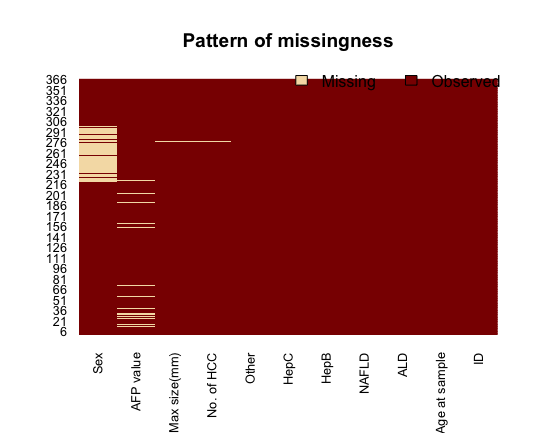
\includegraphics[width=10cm,height=7cm]{Missingness_pattern.png}
    \caption{Missing data pattern in the HCC screening cohort.}
    \label{fig:miss_data}
\end{figure}
\clearpage
\begin{table}[h!] \centering
  \caption{Exploratory analysis of the Screening cohort}
  \label{table:explor1}
\begin{tabular}{@{\extracolsep{5pt}} ccccc}
\\[-1.8ex]\hline
\hline \\[-1.8ex]
 & Aetiologies & Number of patient & Male $\%$ & Mean log AFP  (sd) \\
\hline \\[-1.8ex]
1 & ALL & $1,509$ & 57\% & 0.584 (0.295) \\
2 & ALD & $450$ & 60\% & 0.629 (0.259) \\
3 & NAFLD & $178$ & 58.4\% & 0.6 (0.272) \\
4 & HepC & $403$ & 55.3\% & 0.576 (0.321) \\
5 & HepB & $162$ & 43.8\% & 0.527 (0.263) \\
6 & Other & $453$ & 35.8\% & 0.518 (0.341) \\
\hline \\[-1.8ex]
\end{tabular}
\end{table}
%
\begin{table}[!htbp] \centering
  \caption{Exploratory analysis of the HCC cohort}
  \label{table:explor2}
\begin{tabular}{@{\extracolsep{5pt}} ccccc}
\\[-1.8ex]\hline
\hline \\[-1.8ex]
 & Aetiologies & Number of patient & Male $\%$ & Mean log.AFP (sd) \\
\hline \\[-1.8ex]
1 & ALL & $240$ & 75\% & 1.118 (0.860) \\
2 & ALD & $103$ & 84.5\% & 1.065 (0.791) \\
3 & NAFLD & $61$ & 82\% & 1.106 (1.028) \\
4 & HepC & $7$ & 76.9\% & 0.984 (0.450) \\
5 & HepB & $65$ & 85.7\% & 1.293 (0.947) \\
6 & Other & $61$ & 63.9\% & 1.374 (0.980) \\
\hline \\[-1.8ex]
\end{tabular}
\end{table}
%
%
\section{Literature Review}
\subsection{Background}
\label{sec:background}
The primary aim of this project is to analyse in detail the time until event or survival time for different group and subgroup of the full data set comprising all HCC-free and HCC-diagnosed patients. In survival analysis, the survival time is treated as the response variable which can depend on the combination of other predictors. Survival analysis plays an important role in clinical studies and an important class of relative risk models has been developed. In this project, we are interested in understanding how the risk of HCC development varies in function of the pre-conditional disease of the patient.
\\ \\
We will compare different survival function estimators and determine the optimal approach to adopt by taking into consideration the limitations of these models as well as their advantages and disadvantages.
The most well-known model is the Cox proportional hazards model \cite{cox1992regression} which is a semi-parametric model due to the fact that it does not make any assumption concerning the distribution of the survival times. The model consist of exploring the relationship between the survival time of a patient and the available information we have on this patient (e.g sex, age disease,biomarker level and so on). Once correctly fitted, we can estimate the risk of HCC development based solely one the explanatory variables.
%
%
%
%
%
%
%
%
%------------------------------------------------------------------------------------------------
%------------------------------------------------------------------------------------------------
%
%
%
\subsection{Multivariate Cox Model}
First we need to define two important functions arising in survival analysis, namely the survival and the hazard function.
The survival function is simply expressing the probability of an individual surviving up to a certain time t.
$$S(t) = \Pr[T^*>t]= e^{-H(t)}$$ where $T^*$ denotes the random variable of survival time (in our case the time to diagnosis of HCC) and $H(t)$ the hazard function. The hazard function represents the expected number of event to be observed up to time t which is the sum or accumulated risk up to time t.
\begin{align}
    H(t) &= \int_{0}^{t} h(s) ds \\
    h(t)&=\lim_{dt\to 0} \frac{\Pr[t\leq T^* < t+dt\mid T^* \geq t]}
{dt} \quad \text{,\, $t>0$}
\end{align}
The Cox model is a solid procedure to model the relationship of covariates to an event (failure time or censoring). It assumes a multiplicative effect of covariates on the hazard and specifies the following hazard for an individual i:
\begin{align}
    h_i(t\mid w_i) &=\lim_{dt\to 0} \frac{\Pr[t\leq T^* < t+dt\mid
    T^* \geq t,w_i]}{dt} \\
    &= h_0(t)e^{\gammaw^{T} w_i}
\end{align}
The model can then be decomposed in two parts, a parametric part where $w_i^T=(w_{i1},\dots,w_{ip})$ represents the vector of covariates, $\gamma$ the vector of regression coefficient and a non-parametric part where $h_0(t)$ is an unspecified baseline hazard function (the hazard function when all covariates equal zero).
Analogous to logistic regression, the hazard ratio for one unit change in $w_{ij}$ at any time t is simply $e^{\gamma_j}$.
The estimation of our parameters $\gamma$ in a Cox model are found by partial maximum likelihood (PML). Iterative methods such as Newton-Raphson are then used to solve the PML and obtain the coefficients $\gamma$.
However, risk regression models make several assumptions:
\begin{itemize}
    \item For any two covariates k and l the hazard ratio is constant over time. This is known as the proportional hazards assumption.
        $$\frac{h_0(t\mid w_k)}{h_0(t\mid w_l)}=\frac{h_0(t)e^{w_k}\beta}{h_0(t)e^{w_l}}=e^{w_k-w_l}\beta$$
   \item The distribution of the survival time $T_i^*$ are not specified in the baseline hazard function
   \item The Cox model allow us to take into account all patients even if they were not monitored during the same period or if we did not observe any event (HCC diagnosis) during follow-up (can be used with censoring effect).
\end{itemize}
%
%
%
%------------------------------------------------------------------------------------------------
%------------------------------------------------------------------------------------------------
%
%
%
%
\subsection{Joint Modelling framework}
In the previous two models, we did not take into consideration any time-dependent covariates such as the AFP measures or the age of the patient at each follow-up time. It would,however, be also of interest to investigate the effect of these time-dependent covariates on the associated risk of developing HCC.
\newline
\newline
One possible method would be to extend the Cox model seen previously so that it could handle time-dependent covariates \cite{andersen1982cox}. The issue is that these models can only deal with exogenous covariate  which have the characteristics that the trend of the covariate is not affected by the failure time which is not the case unfortunately for the AFP biomarker. The biomarker is said to be an endogenous variable if its trend is not predictable (due to biological variation and measurement errors). In this case, we cannot  define a survival function conditional on the biomarker's measurements \cite{kalbfleisch2002survival}.
\newline
\newline
To handle time-dependent endogenous covariate an alternative approach known as joint modelling has been proposed.
The aim of this framework is to be able to take into account repeated measurements of the biomarker and to measure any association between the longitudinal data and the hazard of an event  \cite{Rizopoulos2016}.
\\ \\
The joint model can be thought as a two step process. First a longitudinal sub-model, which consists of a linear mixed effect model, is fitted to describe the evolution of the biomarker over time for each patient. Then a survival sub-model,consisting of a simple Cox model, is performed on the wide data set. The joint model evaluates then the joint distribution of the two sub-models.
%
Thus, we first need to define an adequate mixed effect model that will allow us to estimate the true value of the biomarker and reconstruct $M_i(t)$, its longitudinal history. The model has the following general form:
\begin{equation}
\label{eq:MEM}
\left\{\begin{aligned}
y_i(t)&=m_i(t) + \epsilon_i(t),\\
m_i(t)&=x_i^T(t) \beta + z_i^{T}b_i,\\
b_i &\sim N(0,D),\quad \epsilon_i(t) \sim N(0,\sigma^{2}),
\end{aligned}
\right.
\end{equation}
where
\begin{itemize}
    \item $x_i(t)$ and $\beta$ are the Fixed-effects part of the model
    \item $z_i(t)$ and $b_i$ are the Random-effects part of the model
\end{itemize}
Essentially,the mixed effect model allows us to model the response variable $y_i(t)$, the "contaminated" longitudinal response in each subject where each subject has his/her own mean response profile over time. Each individual in this model will have an individual intercept and slope. \\
\\
The fixed effect regression coefficients $\beta=(\beta_1,\dots,\beta_p)$ are interpreted exactly as in a linear regression model. The random effect $b_i$ on the other hand, explains how a subset of the regression parameters for an individual i deviates from those in the population. The random effects follow a multivariate normal distribution with mean zero and covariance matrix D.  Several advantages result from modelling the response variable using mixed models.
\begin{enumerate}
    \item we obtain individual response trajectories
    \item it can accommodate the fact that patients have different number of repeated measurements
\end{enumerate}
%
Next, we need to define a relative risk model for an individual i as follow:
\begin{align*}
    h_i(t \mid M_i(t),w_i) &= h_0(t)e^{\gamma^T w_i + \alpha m_i(t)} \\
    S_i(t\mid M_i(t),\gamma_i) &= \Pr[T_i^* > t\mid M_i(t), \gamma_i] \\
    &= exp \bigg( -\int_{0}^{t}h_0(s) e^{\gamma^T w_i + \alpha\, m_i(s)}\, ds \bigg )
\end{align*}
where
\begin{itemize}
    \item $m_i(t)$ designates the true and observed value of the time-dependent covariate
    \item $M_i(t)$ is the longitudinal measurement history of the biomarker such that \\ $M_i(t) = \{m_i(s),0 \leq s < t$\}
    \item $\alpha$ quantifies the strength of the relationship between AFP values an the risk for an event
    \item $w_i$ ,as before, represents the different predictors at baseline
\end{itemize}
More specifically where $e^{\gamma_i}$ represented the increase of hazard ratio for one unit change in $\gamma_i$, similarly here, $e^{\alpha}$ represents the increase in risk for an event for one unit increase in the true value of AFP level at same time \cite{Rizopoulos2010}. Hence, $\alpha$ as formulated above, determines the strength of the association between the level of AFP at a particular time t and the risk of an event at that same time. This concept can however be extended by re-parameterising the relationship between the longitudinal and survival sub-model. A more complex joint model can then consider not only the AFP level of the biomarker at time t, but also the rate of change of the trajectory at that same time.The survival sub-model becomes then:
\begin{align}
    h_i(t)=h_0(t) e^{\gamma^Tw_i+ \alpha_1m_i(t)+\alpha_2m_i(t)^{'}} \quad
    \text{where}\\
    m_i^{'}=\frac{dm_i(t)}{dt}=\frac{d}{dt}\{x_i(t)\beta+z_i^T(t)b_i\}
\end{align}
In this setup, the model captures not only the difference between two patients with similar AFP levels but also different rate of change at a certain time point. $\alpha_2$ will therefore quantify the association between the slope of the marker and the risk for an event.
\\
\\
%
Finally, the two processes are then combined to form a joint model which has the following general distribution \cite{tsiatis2004joint}:
$$p(T_i,\delta_i,y_i) = \int p(y_i \mid b_i)\{h(T_i \mid b_i)^{\delta_i}
S(T_i\mid b_i)\} p(b_i)\, db_i$$
%
where $S(.)$ denotes the survival function and $p(.)$ the density function.
The estimation procedure can follow two approaches, a frequentist and a Bayesian approach.\\ \\ In the frequentist approach,solving the density and survival function first require the use of numerical integration algorithm (e.g Monte Carlo,Gaussian quadrature). The parameter estimates are then computed via Maximum likelihood and maximisation of the log-likelihood  is evaluated using either the EM algorithm, Newton-Raphson or by a combination of both.
\\ \\
 The estimation of the joint model's parameter under the Bayesian approach is based on Markov Chain Monte Carlo(MCMC) algorithm. Following \cite{sweeting2017using} the main assumptions to derive the posterior distribution is that given the random effects $b_i$, both the longitudinal and survival sub-model are independent such that:
 \begin{align}
     p(\boldsymbol{y_i},T_i,\delta_i \mid \boldsymbol{b_i},\boldsymbol{\theta})&=p(\boldsymbol{y_i}\mid\boldsymbol{b_i},\boldsymbol{\theta})p(T_i,\delta_i\mid\boldsymbol{b_i},\boldsymbol{\theta}),
     \\
     p(\boldsymbol{y_i}\mid\boldsymbol{b_i},\boldsymbol{\theta})&=\prod_l p(y_{il} \mid \boldsymbol{b_i},\boldsymbol{\theta})
 \end{align}
 The second equation assumes that the longitudinal responses between subject are independent. Thus, the posterior distribution is then given by:
 \begin{align}
 \label{eq:posterior}
     p(\boldsymbol{\theta},\boldsymbol{b}) \propto \prod_{i=1}^{n} \prod_{l=1}^{n_i}p(\boldsymbol{y_i}\mid\boldsymbol{b_i},\boldsymbol{\theta})p(T_i,\delta_i\mid\boldsymbol{b_i},\boldsymbol{\theta})p(\boldsymbol{b_i}\mid \boldsymbol{\theta})p(\boldsymbol{\theta})
 \end{align}
 where $p(\boldsymbol{y_i}\mid\boldsymbol{b_i},\boldsymbol{\theta})$ is a member of the exponential family and $p(T_i,\delta_i\mid\boldsymbol{b_i},\boldsymbol{\theta})$ represent the survival part in the joint model. Most parameters can then be updated using Gibbs sampling. However in the case where \ref{eq:posterior} has no conditional posterior closed-form, a Metroplolis -Hasting algorithm is used.
 %
%------------------------------------------------------------------------------------------------
%------------------------------------------------------------------------------------------------
%
%
\section{Results}
\label{sec:Models}
\subsection{MLE estimates of the Cox model}
\label{sec:Simple_cox}
This section illustrates the procedure taken to fit the simple Cox model, a Cox model without time-dependent variable. We will first proceed by fitting multiple univariate relative risk models in order to find the most significant covariates to include in the final survival model. We then use our final adjusted model to run some exploratory analysis such as the estimated distribution of survival time of all patients and  predicted survival curves for the different aetiologies of the patients.  \\ \\
The following analysis was performed using the R package "survival" \cite{therneau2015package}. The data represented a cohort of $1717$ patients with attributes consisting of categorical variables only. For each patients the following attributes were collected: Age at the first sample (categorised into two subsets: $\leq$ median age and $>$ median age), Sex ($0$ for male and $1$ for female, five binary covariates for the presence or not of a pre-conditional disease ALD,NAFLD,Hepatitis B, Hepatitis C and Other. Moreover the status (HCC diagnosed or not) and the time to event (survival time) were recorded as well. Out of the 1717 patients, 211 developed HCC so the occurrence of the event was about $12.3\%$. The median follow up time of the HCC study was 1645 days hence $50\%$ of the patients would have been observed for 1645 days, had there been no events.\\
\\
\subsubsection{Univariate Cox regression models}
%
%
Table \ref{table:univariate_cox} shows the output from seven different univariate Cox regressions.The summary provides the estimates of the regression coefficients and also their statistical significance based on the Wald statistics value ( $z=\frac{\beta}{se(\beta}$). The variable Sex, Age,ALD, NAFLD and HepB have all statistically significant coefficients. \\
\\
We can note that a positive coefficient implies that the risk of developing HCC is higher for patients with greater values. For factor variables (here coded 1 or 0), a negative values suggest that the risk of event for the group coded $1$ relative to the one coded $0$ is lower. Hence, we can deduce from the output that females have a lower risk of developing HCC than males. Similarly, older patient have a lower survival rates than younger ones. \\
\\
The table also shows the hazard ratio which is simply the exponential of the beta coefficient. This gives the effect size of the covariate. For example, patient with ALD have a hazard ratio of around $2$ which suggest that at any particular time, twice as many patient having ALD as a pre-conditional disease are experiencing an event of developing HCC compared to those who not not have ALD. Similarly, female patient the hazard is reduced by a factor of $0.51$ or $49\%$.
%
\begin{table}[!htbp] \centering
  \caption{}
  \label{table:univariate_cox}
\begin{tabular}{@{\extracolsep{5pt}} ccccc}
\\[-1.8ex]\hline
\hline \\[-1.8ex]
 & beta & Hazard Ratio (95\% CI) & Wald test & p-value \\
\hline \\[-1.8ex]
Sex & -0.68 & 0.51 (0.37-0.69) & 19 & 1.4e-05 \\
Age & 1.6 & 5.2 (3.7-7.1) & 99 & 0 \\
ALD & 0.73 & 2.1 (1.6-2.7) & 27 & 2e-07 \\
NAFLD & 1.1 & 3.2 (2.3-4.4) & 47 & 7.7e-12 \\
HepB & -1.3 & 0.27 (0.12-0.6) & 10 & 0.0015 \\
HepC & -0.18 & 0.83 (0.62-1.1) & 1.4 & 0.24 \\
\hline \\[-1.8ex]
\end{tabular}
\end{table}
\subsubsection{Multivariate Cox regression model}
In order to understand how the covariates jointly impact the risk of HCC, we progress to a multivariate Cox regression model. Although the variable HepC was not statistically significant, we still want to compare the predicted survival curves for the different aetiologies and will therefore include it in the model.
\\ \\
Figure \ref{fig:forest_cox} help us visualising the summary of the multivariate Cox model. There is clear evidence from the p-value that all covariates except HepB are statistically significant. \\ \\
We can observe some dramatic change for the new adjusted model. An increase in age is still associated with an increase in risk. The relationship between Sex and HCC diagnosis is almost unaltered after adjustment for Age and all the pre-conditional disease (Hazard ratio CI almost similar before and after adjustment).
On the other hand, after adjustment the hazard ratio for Age, ALD, Other, HepB and HepC considerably increased. Since covariates act as a multiplicative effect in a Cox model and knowing that several patient contracted a combination of aetiologies at follow-up entry, the hazard ratio was very likely to increase when adjusting for additional factors.
%
\begin{figure}[h!]
    \centering
    \includegraphics[width=10cm,height=7cm]{forestplot_true.png}
    \caption{Forestplot of the adjusted Cox proportional hazards model showing the hazard ratio derived from the model for all covariates}
    \label{fig:forest_cox}
\end{figure}
%
Now that the adjusted Cox model is fitted to the data set, we can visualise the distribution of survival times for patient with different aetiologies. Figure \ref{fig:pred_surv_curv_mf} illustrates the predicted survival proportion for the five different pre-conditional disease at any given point in time for males and females.
\begin{figure}[h!]
    \centering
    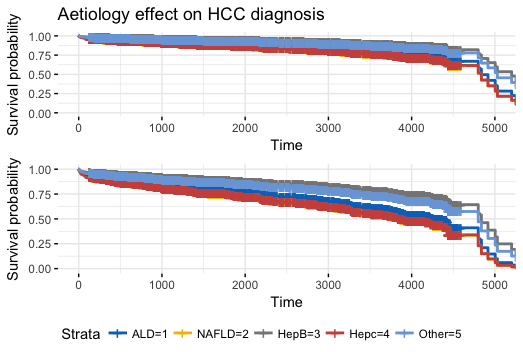
\includegraphics[width=10cm,height=7cm]{Surv_curve_male_female.png}
    \caption{Predicted survival curves for several different aetiologies. Top panel is female patient and bottom panel is male patient}
    \label{fig:pred_surv_curv_mf}
\end{figure}
From the figure, we can see that the survival curve for females are above the one for males since their survival outcome is better relative to the males. In both group, the poorer survival outcome arises for patients with Hepatitis C and NAFLD followed by ALD.\\ \\
%
%------------------------------------------------------------------------------------------------
%------------------------------------------------------------------------------------------------
%
%
\subsection{MCMC estimates of the joint model}
The previous section dealt with categorical and continuous variable that were not time-dependent. We did not use the repeated measurement of the biomarker levels that was recorded for each patient. As previously stated, the extended Cox model offers a way to deal with such covariate but the assumptions made by this type of model cannot be satisfied for endogenous variables. Joint models \cite{laird1982random} offers an alternative framework to work with longitudinal biomarker values by evaluating jointly a survival sub-model with a longitudinal sub-model.
%
To do that, the biomarker measurements were applied a log-transformation so that the AFP levels would be normally distributed \cite{Teofanescu2007}. We restricted our data set for patients with at least two sample measurements. Figure \ref{fig:AFP_dist} illustrates the density shape of the patient's AFP measurements.
%
\begin{figure}[h!]
    \centering
    \begin{subfigure}[t]{0.5\textwidth}
        \centering
        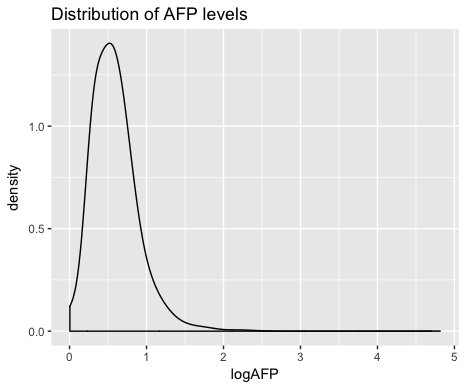
\includegraphics[height=7cm]{All_AFP_levels.png}
        \caption{Distribution of all AFP levels for the 1717 patients.}
    \end{subfigure}%
    ~
    \begin{subfigure}[t]{0.5\textwidth}
        \centering
        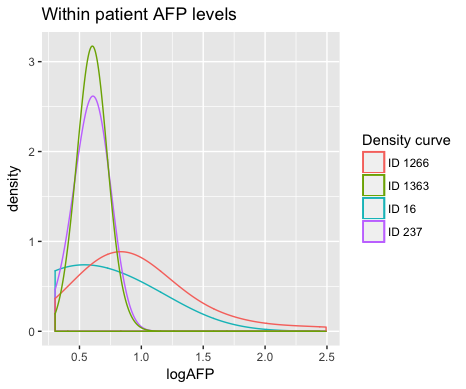
\includegraphics[height=7cm]{Within_patient_AFP.png}
        \caption{Distribution of the AFP levels within each patient for patient with at least 15 measurements}
    \end{subfigure}
    \caption{Distribution of AFP measures}
    \label{fig:AFP_dist}
\end{figure}
 \\ \\
 \subsubsection{The linear mixed-effects model}
 The longitudinal sub-model was constructed using a mixed-effects model which can be simplified to a simple linear mixed-effects model since we are assuming our longitudinal biomarker level to be normally distributed.
 Thus, the following model was fitted using our vector of covariates $\mathbf{x_i^T}=(x_{i1},\dots,x_{i6})$ and $\mathbf{\beta}=(\beta_0,\dots,\beta_7)$:
\begin{equation}
\label{eq:MEM}
\left\{\begin{aligned}
y_i(t)&=m_i(t) + \epsilon_i(t),\\
m_i(t)&=(\beta_0+b_{i0})+(\beta_1+b_{i1})B_n(t,3)+\beta_2\, Sex\\
&+ \beta_3 \, Age_i +\beta_4 \, ALD_i +\beta_5 \, NAFLD_i \\
&+\beta_6 \, HepB_i +\beta_7 \, HepC_i,\\
b_i &\sim N(0,D),\quad \epsilon_i(t) \sim N(0,\sigma^{2}),
\end{aligned}
\right.
\end{equation}
  where $B_n(t,3)$ is a cubic spline, used here to correctly capture $M_i(t)$, especially for subjects with non-linear AFP trajectories (Brown et al,2005)\cite{brown2005flexible} as illustrated in figure \ref{fig:AFP_trend}.\\ \\
  Formulated in that way, it is possible to estimate the parameters that describe how the AFP responses change in the population and it is also possible to predict how individual patient response trajectories change over time. There is no need to specify the specific start and end of the study since the time to event of HCC diagnosis (in days) was, although given, recomputed for each patient. \\ \\
  Indeed, the "JMbayes" package in R \cite{rizopoulos2014r} required that the accumulated observation times (accumulated time elapsed between each sample measurement) be smaller than the survival time. The package logically implied that no further measurements could be taken after a patient 's "death" (here HCC diagnosis). Hence, every measurements for each patient taken after the date of diagnosis were removed. Moreover,patients with left-censored data (patients diagnosed with HCC before entering the study) were also removed from the dataset for simplicity (certain techniques can incorporate left-censored data).
  \begin{figure}[h!]
      \centering
      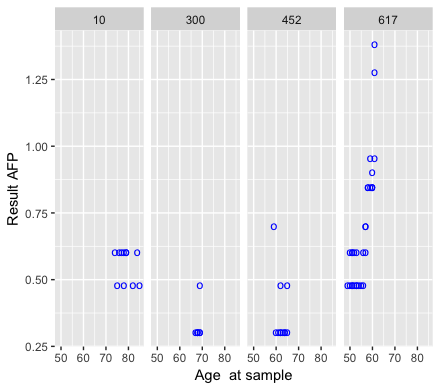
\includegraphics[width=10cm,height=7cm]{AFP_patient_trend_ggplot.png}
      \caption{Subject-specific longitudinal log(AFP) profiles for three patients from the data set}
      \label{fig:AFP_trend}
  \end{figure}
  The estimates for the linear mixed-effects model were derived by maximum likelihood principle, more specifically by Restricted Maximum likelihood (Horvill, 1974) \cite{harville1974bayesian}. \\ \\
  \subsubsection{The time-to-event process}
  For the survival sub-model, we use the result from section \ref{sec:Simple_cox} and fit our Cox survival model in the same way, we have:
  \begin{align}
     h_i(t \mid M_i(t),w_i)&=h_0(t) e^{\boldsymbol{\gamma^{T}w_i}+\alpha_1 m_i(t)+ \alpha_2 \frac{d \, m_i(t)}{dt}} \quad \text{where} \\
     \boldsymbol{\gamma^{T} w_i}&=\gamma_1 \Sex + \gamma_2 \, Age_i +\gamma_3 \, ALD_i +\gamma_4 \, NAFLD_i \\
     &+\gamma_5 \, HepB_i +\gamma_6 \, HepC_i
  \end{align}
 Where $h_0(t)$ denotes the baseline risk function. In our case $h_0(t)$ will correspond to the hazard function of a patient that has $\gamma^T w_i=0$ which correspond to a male patient that entered the study with a pre-conditional disease classified as "Other" as explained in section \ref{sec:Models}. \\ \\
 While in the multivariate Cox model we had the advantage of not having to specified the baseline hazard function to avoid misspecifying the distribution of $T_i^*$, this can unfortunately not be done in the joint modelling framework. This will result in an sever underestimation of the parameter's standard errors \cite{hsieh2006joint}. We can estimate $h_0(t)$ using a estimated risk function computed by non-parametric method so that no assumptions is made on the distribution of the survival times. According to the literature cubic splines approximation are efficient methods bringing increased flexibility in the estimation of the baseline risk function \cite{harrell1984regression}.
 The survival sub-model was parameterised so that the time-dependent slopes of the marker would be also taken into consideration. \\ \\
 %
 The estimation of the joint model's parameter from equation \ref{eq:posterior} was done using the "JMbayes" package which uses a Bayesian approach, proceeding with a Markov Chain Monte Carlo (MCMC) algorithm.More specifically, the MCMC algorithm samples from the posterior conditional parameters and the random effects via a random walk Metropolis-Hastings algorithm \cite{rizopoulos2014r}. The joint model was run using a single chain and without initial values.The chain was run for 20000 iterations with a burn-in of 3000 iterations and a thinning of 10. The acceptance rate for the $\beta$ coefficients (coefficients from the longitudinal sub model) was of $44.5\%$ whereas for the $\gamma$ coefficient of the event process was of $22.93 \%$. The posterior means summary obtained from the MCMC algorithm are shown in table \ref{table:long_post} and \ref{table:event_post}. Figure \ref{fig:MCMC_diagnostics} displayed the density plots of the MCMC chain as well as the convergence of the chain (traceplots).
 \\ \\
 The posterior means for the survival sub-model are displayed in table \ref{table:event_post} and express the log hazard ratio. A negative log hazard ratio is associated with better prognosis. From the table we can then deduce that females have a better prognosis than male which is in accordance with most studies. Out of the six covariates describing the patients characteristics, only the sex variable is negative. From the different aetiologies present in the patients at the start of the study, ALD has the highest value closely followed by Hepatitis C. Hence patient with ALD more than double the hazard compared to baseline (Patient with aetiology categorised as "Other). We can also observed that the intercept of the AFP trajectory (Assoct in table \ref{table:event_post}) is highly associated with the risk for HCC diagnosis (p-value $<< 0.05$). For patient having the same level of AFP, the log hazard ratio for a unit increase in the current intercept of the AFP trajectory is 1.93. Similarly, the rate of change of the AFP levels (AssocE in table \ref{table:event_post}) is also strongly associated with the failure time (p-value = 0.009).
 %
\begin{table}[!htbp] \centering
  \caption{Coefficient estimates for the longitudinal sub-model}
  \label{table:long_post}
\begin{tabular}{@{\extracolsep{5pt}} ccccccc}
\\[-1.8ex]\hline
\hline \\[-1.8ex]
 & Value & Std.Err & Std.Dev & 2.5\% & 97.5\% & P \\
\hline \\[-1.8ex]
(Intercept) & $0.210$ & $0.002$ & $0.022$ & $0.167$ & $0.250$ & $0$ \\
ns(Obstime, 3)1 & $-0.052$ & $0.001$ & $0.019$ & $-0.090$ & $-0.015$ & $0.007$ \\
ns(Obstime, 3)2 & $-0.135$ & $0.001$ & $0.020$ & $-0.174$ & $-0.097$ & $0$ \\
ns(Obstime, 3)3 & $-0.066$ & $0.002$ & $0.024$ & $-0.114$ & $-0.019$ & $0.007$ \\
Sex & $0.007$ & $0.001$ & $0.020$ & $-0.033$ & $0.047$ & $0.685$ \\
Age & $0.007$ & $0.00004$ & $0.0002$ & $0.007$ & $0.008$ & $0$ \\
ALD & $0.095$ & $0.001$ & $0.024$ & $0.050$ & $0.142$ & $0$ \\
NAFLD & $0.021$ & $0.001$ & $0.030$ & $-0.039$ & $0.080$ & $0.458$ \\
HepB & $-0.014$ & $0.001$ & $0.034$ & $-0.080$ & $0.052$ & $0.684$ \\
HepC & $0.098$ & $0.001$ & $0.017$ & $0.064$ & $0.130$ & $0$ \\
\hline \\[-1.8ex]
\end{tabular}
\end{table}
%
\begin{table}[!htbp] \centering
  \caption{Coefficient estimates for the Cox survival sub-model}
  \label{table:event_post}
\begin{tabular}{@{\extracolsep{5pt}} ccccccc}
\\[-1.8ex]\hline
\hline \\[-1.8ex]
 & Value & Std.Err & Std.Dev & 2.5\% & 97.5\% & P \\
\hline \\[-1.8ex]
Sex & $-0.837$ & $0.013$ & $0.183$ & $-1.188$ & $-0.476$ & $0$ \\
Age & $0.095$ & $0.002$ & $0.007$ & $0.080$ & $0.106$ & $0$ \\
ALD & $0.789$ & $0.011$ & $0.159$ & $0.494$ & $1.117$ & $0$ \\
NAFLD & $0.533$ & $0.013$ & $0.198$ & $0.136$ & $0.922$ & $0.001$ \\
HepB & $0.298$ & $0.032$ & $0.446$ & $-0.603$ & $1.126$ & $0.510$ \\
HepC & $0.771$ & $0.016$ & $0.192$ & $0.382$ & $1.154$ & $0$ \\
Assoct & $1.930$ & $0.005$ & $0.094$ & $1.747$ & $2.111$ & $0$ \\
AssoctE & $0.252$ & $0.079$ & $3.102$ & $-5.954$ & $6.225$ & $0.009$ \\
tauBs & $66.612$ & $8.017$ & $71.051$ & $3.522$ & $259.697$ &  \\
\hline \\[-1.8ex]
\end{tabular}
\end{table}
\begin{figure}
    \centering
    \includegraphics[width=10cm,height=7cm]{MCMC_joinModel.png}
    \caption{Density plots and traceplots of the MCMC chain for each parameter of the survival sub-model.}
    \label{fig:MCMC_diagnostics}
\end{figure}
 \\ \\
 \subsubsection{Dynamic predictions using the joint model}
 From the Bayesian estimates, the joint model can be used to make dynamic predictions for future biomarker levels for each individual patient in the study. Moreover, individual survival probabilities can be computed too. Figure \ref{fig:Dynpred1} and \ref{fig:Dyn_pred2} illustrates two predictions made on two different patients based on their AFP measurements and characteristics. Patient number $407$ was in the screening cohort and did not developed HCC. We can see that the patient's AFP levels were decreasing over time hence we can see that the patient 's chance of survival increased by about $10\%$ on a five year and a half timescale. On the other hand, for the second patient (patient number "L170") who was in the HCC screening cohort and did develop HCC, his/her AFP levels dramatically increased over time hence lowering his chance of not getting HCC. By the end of the first year, his/her chance of "survival" were already close to $0$.
 %
 \begin{figure}[h!]
    \centering
    \includegraphics[width=10cm,height=7cm]{dynmaic_pred_739.png}
    \caption{Dynamic predictions of survival probabilities for patient in the screening cohort who did not develop HCC. The vertical dot line represent the time point of the last AFP measurement. On the left side of the vertical line is represented the longitudinal trajectories. On the right, the predicted survival curve with the red line representing the mean survival rate with a $95\%$ pointwise confidence interval.}
    \label{fig:Dynpred1}
\end{figure}
\begin{figure}[h!]
    \centering
    \includegraphics[width=10cm,height=7cm]{Dynpred_L170_2.png}
    \caption{Dynamic predictions of survival probabilities for patient in the HCC screening cohort who developed HCC. The vertical dot line represent the time point of the last AFP measurement. On the left side of the vertical line is represented the longitudinal trajectories. On the right, the predicted survival curve with the red line representing the mean survival rate with a $95\%$ pointwise confidence interval.}
    \label{fig:Dyn_pred2}
\end{figure}
%
%
%%
%
% %
\clearpage
%
%
%
\section{Discussion and limitations}
\subsection{Discussion}
\label{sec:Discussion}
By using the data from a well-defined cohort of ongoing HCC-free patients undergoing regular HCC surveillance and a cohort of patients diagnosed with HCC, we observed differences in the risk of HCC development in populations with different causes of liver disease. In this project, we illustrated the different survival times between male and female who entered the study with a specific pre-conditional disease. \\ \\
We initially postulated a multivariate Cox model without including the AFP measures. The results suggested that both age and sex were statistically significant variables that were affecting the hazard ratio of HCC diagnosis. The results also suggested that among the five aetiologies directly linked with liver cancer,patients with ALD and NAFLD were associated with worst prognosis than those with hepatitis B,C or other forms of disease. Figure \ref{fig:pred_surv_curv_mf} showed a significant drop of the survival probabilities for male patient diagnosed with ALD and NAFLD compared to female patients within the same subgroup. Hence, our results indicate that the male/female gender bias in HCC development is stronger for patients with ALD and NAFLD rather than patients with viral infections or autoimmune diseases. \\ \\
%
In our second approach, we used a joint model framework to extend the multivariate Cox model and therefore taking into consideration the longitudinal measurements of the AFP biomarker. With this method we jointly evaluated a survival and a linear mixed-effects model and associated the biomarker true value and rate of change at a certain point in time with the risk of developing HCC. The results were in accordance with the first model and coefficients for the survival sub-model were similar. The joint model accentuated the better prognosis for female patients compared to the one for male and and reduced the hazard of a HCC diagnosis from 2.75 to 1.7 fold for patient with NAFLD. We showed the current level of the AFP measure and its rate of change was strongly associated with the risk of cancer diagnosis. The results allowed us to provide individualised predictions for the survival and longitudinal outcomes as illustrated in figure \ref{fig:Dynpred1} and \ref{fig:Dyn_pred2}.
%%%
%
\subsection{Limitations}
Throughout this project, we did not emphasize on the predictive performance of any fitted model, nor did we analytically evaluate their prospective accuracy. The reason is that we assume a non-informative censoring mechanism when evaluating the survival models.Namely, we hypothesize the fact that a patient withdrawing from the study for reasons completely unrelated to his/her prognosis. This can be seen as a "missing completely at random" mechanism (MCAR) that we found in longitudinal studies where statistical methods have been develop to efficiently deal with them. However, in our case, we considered every patient in the cohort study who did not develop HCC as right censored data and assumed that they simply did not experience an event or randomly left the study. The problem is, that most patients who did leave the study, did so \textbf{because} they did not develop liver cancer in the future. Hence, the probability of a subject being censored depends on the failure process and we have an informative censoring mechanism. \\ \\
Therefore, the main idea of the project was to perform mainly exploratory analysis using the HCC and HCC-free patient's data and to suggest an adequate methodology to adopt should the data be taken in a randomised trial or in another set up making sure that the censoring process is unrelated to the failure rates. Indeed, non-informative censoring mechanism produces highly biased results and the estimates obtained in this study should not reflect the true risk of HCC diagnosis. Similarly, the predicted survival probabilities serve here as an illustrative purpose. \\ \\
%
%
\section{Conclusion}
%
%
%
In this report we have described two different survival analysis approaches to estimate the survival probabilities of patients suffering from different pre-conditional diseases in the Lothian region. \\ \\
From our result, we have been able to identify the different risk factors associated with each aetiologies. We showed that the gender and the age of a patient were statistically significant predictors of the two survival models.
\\ \\ According to the multivariate Cox model, ALD,NAFLD and Hepatitis C suffering patients were the one more at risk of developing HCC. The median survival time of these patient was about nine years and a half for males while Hepatitis B suffering patients and patients with autoimmune disease such as PBC and haemochromatosis, had a median survival time of around thirteen years. This represents a four years difference that could be crucial for the treatment of early stage liver cancer. Our results also shown that the gender bias in developing HCC is more pronounced in ALD, NAFLD and Hepatitis C compared to the other aetiologies.  \\ \\
In addition, we proposed an alternative framework to assess the patient's risk of developing HCC. We derived a joint model that took into consideration the AFP levels of each patient which can then predict the survival probabilities of the patient after each new measurement. For further study, it would be interesting to use the joint model to select the optimal time point to plan the next measurement. This could dramatically reduce the cost of unnecessary screening tests and biopsy operations.
\\ \\
To conclude, we recommend monitoring closely patients aged equal to or above the median age of the cohort and suffering from ALD, NAFLD or Hepatitis C. This could be done by using our derived joint model that allow to constantly update the prediction of the patient's survival probabilities.
\clearpage

% the entries have to be in the file literature.bib
\bibliographystyle{unsrt}
\bibliography{library}
\clearpage

\appendix
\section*{R codes}
\addcontentsline{toc}{section}{Appendices}
\begin{lstlisting}

## Loading the libraries


rm(list = ls())
if (!require(tidyverse)) install.packages('tidyverse'); require(tidyverse)
if (!require(ggplot2)) install.packages('ggplot2'); require(ggplot2)
if (!require(reshape2)) install.packages('reshape2'); require(reshape2)
if (!require(gridExtra)) install.packages('gridExtra'); require(gridExtra)
if (!require(rjags)) install.packages('rjags'); require(rjags)
if (!require(stargazer)) install.packages('stargazer'); require(stargazer)
if (!require(ggfortify)) install.packages('ggfortify'); require(ggfortify)
if (!require(ggmcmc)) install.packages('ggmcmc'); require(ggmcmc)
if (!require(metRology)) install.packages('metRology'); require(metRology)
if (!require(fBasics)) install.packages('fBasics'); require(fBasics)
if (!require(gridExtra)) install.packages('gridExtra'); require(gridExtra)
if (!require(xtable)) install.packages('xtable'); require(xtable)
if (!require(JM)) install.packages('JM'); require(JM)
if (!require(JMbayes)) install.packages('JMbayes'); require(JMbayes)
if (!require(rstan)) install.packages('rstan'); require(rstan)
if (!require(lme4)) install.packages('lme4'); require(lme4)
if (!require(readxl)) install.packages('readxl'); require(readxl)
if (!require(lubridate)) install.packages('lubridate'); require(lubridate)
if (!require(readxl)) install.packages('readxl'); require(readxl)
if (!require(lubridate)) install.packages('lubridate'); require(lubridate)

############################################################################
#-------------------------------------HCC in screening dataset ------------
############################################################################
############################################################################

# Load the HCC in screening dataset from computer
HCC.data <-read_excel("HCC_in_screening_clean.xlsx",sheet = "Sheet1",
                      col_types = c("text","numeric","date",
                      rep("numeric",8),"date","numeric","numeric"))

# reorder dataframe
HCC.data <- HCC.data[order(HCC.data$ID),]
## cleaning the data
count.HCC <- HCC.data %>% group_by(ID) %>%
  summarize(count=n())
#check ordering
stopifnot(count.HCC$ID==unique(HCC.data$ID))

#Impute values into long format
sex.HCC <- HCC.data %>%  dplyr::select(Sex)%>%
  filter(Sex!="NA")
aetiology.HCC <- HCC.data %>%dplyr:: select(ALD:Other) %>%
  filter_all(all_vars(.!='NA'))
HCC.data$Sex <- rep(sex.HCC$Sex,times=count.HCC$count)
for (i in 1:dim(aetiology.HCC)[2]){
  HCC.data[,6+i] <- rep(pull(aetiology.HCC[,i]),
                        times=count.HCC$count)
}

# Add status (event)
HCC.data$Status <- rep(1,length(HCC.data$ID))

# Add observation time (time point for each measurements) per patient
Obstime <- list()
obstime.temp <- NULL
for (i in unique(HCC.data$ID)){
  for (j in 1:count.HCC$count[count.HCC$ID==i]){
    patient.dates <- HCC.data$"Sample_date"[HCC.data$ID==i]
    init.date <- patient.dates[1]
    obstime.temp[j] <- difftime(patient.dates[j],init.date,units = "days")
  }
  Obstime[[i]] <- obstime.temp
  obstime.temp <- NULL
}

HCC.data$Obstime <- unlist(Obstime)

# Recalculate time to event
data.sample.temp <- HCC.data %>% group_by(ID) %>%
  filter(row_number(ID) == 1)
date.sample <- ymd(as.character(data.sample.temp$Sample_date))
start.date <- date.sample[!is.na(date.sample)]
date.diagnosis <- ymd(as.character(HCC.data$Diagnosis))
end <- date.diagnosis[!is.na(date.diagnosis)]

time.to.event <- difftime(end,start.date,units="days")
HCC.data$TimeEvent <- rep(time.to.event,times=count.HCC$count)

# Remove NAN
HCC.temp1 <- HCC.data%>% dplyr::select(ID,Sex,Age_sample,Time,
                                       AFP,ALD:Other,
                                       Status,Obstime,TimeEvent)%>%
  filter_all(all_vars(.!='NA'))

# rename column
colnames(HCC.temp1)[colnames(HCC.temp1)=='Age_sample']<- 'Age'
colnames(HCC.temp1)[colnames(HCC.temp1)=='HEPC'] <- 'HepC'

#remove left censored event
HCC.temp2 <- HCC.temp1%>%dplyr:: select(ID,Sex,Age,AFP,Time,
                                        ALD:Other
                                        ,Status,Obstime,
                                        TimeEvent)%>%
  filter_at(vars(TimeEvent), any_vars(.>0))

#Remove longitudinal measurements after event/diagnosis
HCC.temp3 <- HCC.temp2%>%dplyr:: select(ID,Sex,Age,Time,
                                        AFP,ALD:Other
                                        ,Status,Obstime,
                                        TimeEvent)%>%
  filter_at(vars(Time), any_vars(.<0))

# check that TimeEvent > Obstime
stopifnot(HCC.temp3$TimeEvent > HCC.temp3$Obstime)

indices <-which(HCC.temp3$TimeEvent< HCC.temp3$Obstime)
# remove
HCC.temp3 <- HCC.temp3[-indices,]

HCC.data <- HCC.temp3 %>% dplyr:: select(ID,Sex,Age,AFP,
                                         ALD:Other
                                         ,Status,Obstime,
                                         TimeEvent)

###############################################################
#--------------- Cohort in screening dataset------------------
###############################################################
###############################################################

df.JM <- read_excel("Screening_cohort_clean.xlsx",sheet = 1,
                    col_types = c("text",rep("numeric",13)))

# set time at sample
df.JM$Obstime <- df.JM$Sample_time-df.JM$Time

# Add censoring status
df.JM$Status <- rep(0,length(df.JM$ID))

# Select important covariates
data.JM.cohort <- df.JM %>% dplyr::select(ID:Age,
                                          Time,ALD:Other,AFP,Obstime,Status)

# Filter patients with at least two measurements
df.JM.temp <- data.JM.cohort %>% group_by(ID) %>%
  filter(n() >= 2)

#Change sign of Time to event
df.JM.temp$Time <- as.numeric(-df.JM.temp$Time)

# rename column
colnames(df.JM.temp)[colnames(df.JM.temp)=='Time']<-'TimeEvent'


#Filter NA values
df.JM.temp <- df.JM.temp %>% dplyr::select(ID:Age,
                                           TimeEvent,ALD:Other,
                                           AFP,Obstime,Status) %>%
  filter_all(all_vars(.!='NA'))

#remove left censored event
df.JM.temp2 <- df.JM.temp %>% dplyr:: select(ID:Age,TimeEvent,
                                             ALD:Other,AFP,Obstime,
                                             Status)%>%
  filter_at(vars(TimeEvent), any_vars(.>0))

# check that Time >= Obstime
stopifnot(df.JM.temp2$TimeEvent >= df.JM.temp2$Obstime)

# Remove inconsitencies in data reporting
JM.cohort <- df.JM.temp2 %>% dplyr::select(ID:Age,
                                           TimeEvent,ALD:Other,
                                           AFP,Obstime,Status)%>%
  filter_at(vars(Obstime), any_vars(.>=0))

#------------------Joining the two datasets ---------------

full.data.long <- bind_rows(HCC.data,JM.cohort)

# check that Time >= Obstime
stopifnot(full.data.long$TimeEvent >= full.data.long$Obstime)




#################################################################
#################################################################
#----------------------PArt I - Cox model---------------------


# Loading the cleaned dataset
df.long <- read_excel("Full_data_final.xlsx",sheet = 1,
                      col_types = c("text",rep("numeric",11)))
df.wide <- df.long[!duplicated(df.long$ID),]

## a) ---------- Unadjusted Cox regression models ----

# Univariate Cox regression

covariates <- c("Sex","Age","ALD", "NAFLD", "HepB","HepC","Other")
univ.formulas <- sapply(covariates,
                        function(x) as.formula(paste('Surv(TimeEvent,
                                                     Status)~', x)))

univ.models <- lapply( univ.formulas,
                       function(x){coxph(x, data = df.wide)})

# Extract summary for each univariate model
univ.results<-lapply(univ.models,
                       function(x){
                         x <- summary(x)
                         p.value<-signif(x$wald["pvalue"],
                                         digits=2)
                         wald.test<-signif(x$wald["test"],
                                           digits=2)
                         beta<-signif(x$coef[1],
                                      digits=2);#coeficient beta
                         HR <-signif(x$coef[2],
                                     digits=2);#exp(beta)
                         HR.confint.lower <- signif(x$conf.int[,"lower .95"], 2)
                         HR.confint.upper <- signif(x$conf.int[,"upper .95"],2)
                         HR <- paste0(HR, " (",
                                      HR.confint.lower, "-", HR.confint.upper, ")")
                         res<-c(beta, HR, wald.test, p.value)
                         names(res)<-c("beta", "HR (95% CI for HR)", "wald.test",
                                       "p.value")
                         return(res)
                         #return(exp(cbind(coef(x),confint(x))))
                       })
res <- t(as.data.frame(univ.results, check.names = FALSE))
univ.res <- as.data.frame(res)
stargazer(univ.res)

## b) ---------- Multivariate Cox regression model --------

res.cox <- coxph(Surv(TimeEvent, Status) ~ Sex+age.cat+ALD+NAFLD+HepB+HepC,
                 data =df.wide)
sum.res.cox <- summary(res.cox)
stargazer(sum.res.cox$coefficients,summary = FALSE)
cox.zph(res.cox, transform="km", global=TRUE)

# Diagnostic plots

par(mfrow=c(2, 2))
plot(cox.zph(res.cox))
ggforest(res.cox)
#Systematic departures from a horizontal line are indicative of
#non-proportional hazards


#Estimated Survival Function Distribution
ggsurvplot(survfit(res.cox), color = "#2E9FDF",
           ggtheme = theme_minimal(),data = df.wide)

#assess the impact of the sex on the estimated survival probability

# Create the new data
aetiologies.df <- with(df.wide,
                       data.frame(Sex = c(1, 1,1,1),
                                  ALD = c(1,0,0,0),
                                  NAFLD = c(0,1,0,0),
                                  HepB = c(0,0,1,0),
                                  Other = c(0,0,0,1)))

# predicted survival curves
fit <- survfit(res.cox, newdata = aetiologies.df)
ggsurv <- ggsurvplot(fit,data = df.wide, conf.int = FALSE,
                     legend.labs=c("ALD=1", "NAFLD=2",
                                   "HepB=3","Other=4"),
                     ggtheme = theme_minimal()) +
  ggtitle("Pre-conditional disease impact")

#############################################################

#############################################################
#------------- Joint Modelling ------------------------------

#Load dataset
full.data.long <- read_excel("Full_data_final.xlsx",sheet = 1,
                      col_types = c("text",rep("numeric",11)))

## sorting the data for the Joint Model
sortnames <- c("ID","TimeEvent")
DATA.long <- full.data.long[do.call("order", full.data.long[sortnames]),]
DATA.wide <- DATA.long[!duplicated(DATA.long$ID),]

##------------------Model I -------------
lmefit1 <- lme(AFP~ns(Obstime,2)+Sex+Age,random = ~ns(Obstime,2)|ID,
               data = DATA.long)
coxfitA <- coxph(Surv(TimeEvent,Status)~Sex+ALD+NAFLD+HepC+Other,
                 data = DATA.wide,x=TRUE)

jointFit1 <- jointModelBayes(lmefit1,coxfitA,
                             timeVar = "Obstime",n.iter=10000,n.burnin=1000)

jointFitBayes <- jointModelBayes(lmeFit, coxFit,
                                 timeVar = "Obstime",baseHaz ="P-splines")

##------------------Model II --------------

lmefit2 <- lme(AFP~ns(Obstime,2)+Sex+Age+ALD+NAFLD+HepB+HepC,
               random = ~ns(Obstime,2)|ID,
               data = DATA.long)
coxfitB <- coxph(Surv(TimeEvent,Status)~Sex+ALD+NAFLD+HepB+HepC,
                 data = DATA.wide,x=TRUE)

jointFit2 <- jointModelBayes(lmefit2,coxfitB,timeVar = "Obstime")
summary(jointFit2)
stargazer(summary(jointFit2),summary = FALSE)
plot(jointFit2)

joinfit2 <- jointModel(lmefit2,coxfitB,timeVar = "Obstime")
summary(jointfit2)
plot(jointfit2)

##-------------------------------Model III -----------------
# No splines or polynomials
ctrl <- lmeControl(opt='optim')
lmefit3 <- lme(AFP~Obstime+Sex+Age+ALD+NAFLD+HepB+HepC,
               random = ~Obstime|ID,
               data = DATA.long)

coxfit3 <- coxph(Surv(TimeEvent,Status)~Sex+ALD+NAFLD+HepC,
                 data = DATA.wide,x=TRUE)

jointFit3 <- jointModelBayes(lmefit3,coxfit3,timeVar="Obstime",
                             parameterization="both",derivForm=dform)

summary(jointFit3)

# Parametrization:
dForm <- list(fixed~0+dns(Obstime,2),random=~0+dns(Obstime,2),
              indFixed=2:3,indRandom=2:3)

joinFit3.update <- update(jointFit1,param="td-extra",extraForm=dForm)

summary(jointFit3.update)
plot(jointFit3.update)


# add parametrization (slope + intercept)
dForm <- list(fixed=~0+dns(Obstime,2),random=~0+dns(Obstime,2),
              indFixed=2:3,indRandom=2:3)

joinFit2.update <- update(jointFit2,param="td-both",extraForm=dForm)
summary(joinFit2.update)
plot(jointFit2)

# add parametrization random effect

joinFit2.update2 <-update(jointFit2,param="shared-RE")
summary(joinFit2.update2)
plot(joinFit2.update2)


##--------------Model IV - Final Model ----------

ctrl <- lmeControl(opt='optim')
lmefit4 <- lme(AFP~ns(Obstime,3)+Sex+Age+ALD+NAFLD+HepB+HepC,
               random = list(ID=pdDiag(form=~ns(Obstime,3))),
               data = DATA.long)

coxfit4 <- coxph(Surv(TimeEvent,Status)~Sex+Age+ALD+NAFLD+HepB+HepC,
                 data = DATA.wide,x=TRUE)

jointFit4 <- jointModelBayes(lmefit4,coxfit4,timeVar="Obstime")

summary(jointFit4)


#Add parameterization
dForm4 <- list(fixed=~0+dns(Obstime,3),random=~0+dns(Obstime,3),
               indFixed=2:4,indRandom=2:4)

joinFit4.update <- update(jointFit4,param="td-both",extraForm=dForm4)

sum.joinFit4 <- summary(joinFit4.update)

stargazer(sum.joinFit4$`CoefTable-Long`)
stargazer(sum.joinFit4$`CoefTable-Event`)

# Diagnostic plot
density.variables <- as.data.frame(joinFit3.update$mcmc$gammas)
density.variables$iterations <- 1:2000

#density plots

a <- ggplot(density.variables, aes(x=ALD)) +
  geom_density(fill="lightblue")

b <- ggplot(density.variables, aes(x=NAFLD)) +

  geom_density(fill="lightblue")
c <- ggplot(density.variables, aes(x=HepB)) +

  geom_density(fill="lightblue")
d <- ggplot(density.variables, aes(x=HepC)) +

  geom_density(fill="lightblue")

#traceplots
aa <- ggplot(data=density.variables,aes(x=iterations,y=ALD))+geom_line()
bb <- ggplot(data=density.variables,aes(x=iterations,y=NAFLD))+geom_line()
cc <- ggplot(data=density.variables,aes(x=iterations,y=HepB))+geom_line()
dd <- ggplot(data=density.variables,aes(x=iterations,y=HepC))+geom_line()


# Subplots
grid.arrange(a,aa,b,bb,c,cc,d,dd,top="Survival sub-model coefficients",
             left="density plots", right="traceplots",ncol=2)


# Survival probability for patient L170
data <- DATA.long[DATA.long$ID=="L170",]

# PLot the data
sfit3 <- survfitJM(joinFit4.update,newdata=data[1,],idVar = "ID")
sfit4 <- survfitJM(joinFit4.update,newdata=data[1:3,],idVar = "ID")
sfit5 <-  survfitJM(joinFit4.update,newdata=data[1:nrow(data),],idVar = "ID")

par(mfrow=c(1,3))
plotfit3 <- plot(sfit3,estimator="mean",include.y=TRUE,
                 conf.int=0.95,fill.area=TRUE,col.area="lightblue",
                 main="patient L170")
plotfit4 <- plot(sfit4,estimator="mean",include.y=TRUE,
                 conf.int=0.95,fill.area=TRUE,col.area="lightblue",
                 main="patient L170")
plotfit5 <- plot(sfit5,estimator="mean",include.y=TRUE,
                 conf.int=0.95,fill.area=TRUE,col.area="lightblue",
                 main="patient L170")


\end{lstlisting}
\end{document}
